\documentclass[12pt]{article}


\usepackage{amssymb}
\usepackage{amsmath}
\usepackage{fullpage}
\usepackage{epsfig}
\usepackage{epstopdf}
\everymath{\displaystyle}

\newif\ifans

\anstrue

\begin{document}

\begin{center}
\underline{\LARGE{Chapters 2.3 \& 2.4 Practice Problems}}
\end{center}

\noindent EXPECTED SKILLS:

\begin{itemize}

\item Know that the derivative of a constant function is 0.

\item Be able to compute the derivatives of sums, differences, and constant multiples of functions.

\item Know how to compute the derivatives of power functions by using the Power Rule.

\item Be able to compute higher order derivatives.

\item Know how to compute the derivatives of products and quotients of differentiable functions by correctly applying the product and quotient rules, respectively.

\end{itemize}

\noindent PRACTICE PROBLEMS:

\medskip

\begin{enumerate}

\item Differentiate.

\begin{enumerate}

\item $f(x)=167.9$

\ifans{\fbox{$f^{\prime}(x)=0$}} \fi

\item $f(x)=x^4+6$

\ifans{\fbox{$f^{\prime}(x)=4x^3$}} \fi

\item $y=x^2-4x$

\ifans{\fbox{$\displaystyle \frac{dy}{dx}=2x-4$}} \fi

\item $y=2x-4x^3$

\ifans{\fbox{$y^{\prime}=2-12x^2$}} \fi

\item $f(x)=-x^5+3x^4-2x^3+3$

\ifans{\fbox{$y^{\prime}=-5x^4+12x^3-6x^2$}} \fi

\item $y=\sqrt{x}$

\ifans{\fbox{$\displaystyle y^{\prime}=\frac{1}{2\sqrt{x}}$}} \fi

\item $\displaystyle f(x)=\sqrt[3]{x^7}$

\ifans{\fbox{$\displaystyle \frac{dy}{dx}=\frac{7}{3}x^{4/3}$}} \fi

\item $f(x)= \pi^3+e^2-\sqrt{2}$

\ifans{\fbox{$\displaystyle f^{\prime}(x)=0$}} \fi

\item $\displaystyle y=\frac{3}{x}-\frac{4}{5x^2}$

\ifans{\fbox{$\displaystyle y^{\prime}=-\frac{3}{x^2}+\frac{8}{5x^3}$}} \fi

\item $\displaystyle f(x)=\left(4x^2-\frac{1}{3x}\right)\left(\frac{1}{x^2}\right)$

\ifans{\fbox{$\displaystyle f^{\prime}(x)=\frac{1}{x^4}$}} \fi

\end{enumerate}

\item Find $\displaystyle \left.\frac{dy}{dx}\right|_{x=1}$ if $y=(x^2-1)(3x^2+2)$

\ifans{\fbox{$\displaystyle \left.y^{\prime}\right|_{x=1}=10$}} \fi

\item Let $f(0)=3$, $f^{\prime}(0)=7$, $g(0)=2$, and $g^{\prime}(0)=5$.  Compute each of the following:

\begin{enumerate}

\item $\left(f+g\right)^{\prime}(0)$

\ifans{\fbox{12}} \fi

\item $\left(fg \right)^{\prime}(0)$

\ifans{\fbox{29}} \fi

\item $\displaystyle \left(\frac{f}{g}\right)^{\prime}(0)$

\ifans{\fbox{$\displaystyle -\frac{1}{4}$}} \fi

\end{enumerate}

\item Consider $h(x)=x^2f(x)$.  Compute $h^{\prime}(3)$ if $f(3)=1$ and $f^{\prime}(3)=4$.

\ifans{\fbox{42}} \fi

\item Consider $y=\sqrt{x}f(x)$.  Compute $\displaystyle \left.\frac{dy}{dx}\right|_{x=16}$ if $f(16)=2$ and $f^{\prime}(16)=5$.

\ifans{\fbox{20.25}} \fi

\item Compute an equation of the line which is tangent to $\displaystyle y=\frac{x^3}{f(x)}$ at $x=2$ if $f(2)=3$ and $f^{\prime}(2)=4$

\ifans{\fbox{$\displaystyle y-\frac{8}{3}=\frac{4}{9}(x-2)$}} \fi

\item Find all value(s) of $x$ for which $f(x)=x^3-4x^2$ has horizontal tangent lines.

\ifans{\fbox{$x=0$ and $\displaystyle x=\frac{8}{3}$}} \fi

\item Find all value(s) of $x$ at which the tangent line(s) to $y=x^2+3$ are parallel to $y=7x$.

\ifans{\fbox{$\displaystyle x=\frac{7}{2}$}} \fi

\item Find all value(s) of $x$ for which the tangent line(s) to $\displaystyle y=\frac{x+2}{x+1}$ are perpendicular to $y=x$.

\ifans{\fbox{$x=0$ or $x=-2$}} \fi

\item Find all value(s) of $x$ at which the tangent line to $\displaystyle f(x)=\frac{1}{x+3}$ passes through the origin.

\ifans{\fbox{$\displaystyle -\frac{3}{2}$}} \fi

\item Let $f(x)=x^3-3x+1$.  Determine $f^{\prime \prime}(x)$

\ifans{\fbox{$6x$}} \fi

\item Consider $\displaystyle y=\frac{1}{x}$.  What is $y^{\prime \prime}$?

\ifans{\fbox{$\displaystyle \frac{2}{x^3}$}} \fi 

\item Suppose $\displaystyle f(x)=\frac{3x}{x-3}$.  Compute $\displaystyle \frac{d^2y}{dx^2}$

\ifans{\fbox{$\displaystyle \frac{18}{(x-3)^3}$}} \fi

\item Let $\displaystyle f(x)=\frac{x+1}{x}$.  Determine $f^{\prime \prime}(x)$.

\ifans{\fbox{$\displaystyle \frac{2}{x^3}$}} \fi 

\item Consider $y=x^{80}-17x^5+100x^2-1$.  What is $\displaystyle \frac{d^{81}y}{dx^{81}}$.

\ifans{\fbox{0}} \fi 

\item Let $f(x)=x^3$.  Compute all value(s) of $x$ in $(1,3)$ at which the tangent line to the graph of $f(x)$ is parallel to the secant line which cuts the curve at $x=1$ and $x=3$.

\ifans{\fbox{$\displaystyle x=\sqrt{\frac{13}{3}}$}} \fi

\item {\bf Multiple Choice:} Let $f(x)=ax^2+bx+c$, where $a$, $b$, and $c$ are constants.  Also, suppose that $f(2)=4$, $f^{\prime}(2)=-3$, and $f^{\prime \prime}(2)=-2$.  Find $\frac{a+b+c}{3}$.

\begin{enumerate}

\item $-2$

\item $-1$

\item $0$

\item $1$

\item $2$

\end{enumerate}

\ifans{\fbox{e}} \fi

\item Let $n$ be a positive integer and $\displaystyle f(x)=\frac{1}{x^n}$.  Use the quotient rule to show that $f^{\prime}(x)=-nx^{-n-1}$.

\ifans{\fbox{$\displaystyle f^{\prime}(x)=\frac{(x^n)(0)-(1)(nx^{n-1})}{(x^n)^2}=-\frac{nx^{n-1}}{x^{2n}}=-nx^{-n-1}$}} \fi

\item Let $\displaystyle f(x)=\frac{2}{x}$

\begin{enumerate}

\item Compute an equation of the tangent line to $f(x)$ at $x=1$.

\ifans{\fbox{$y=-2x+4$}} \fi

\item Sketch $f(x)$ and the segment of the tangent line (from part a) which is in the first quadrant.  Label the $x$ and $y$ intercepts.

\ifans{\fbox{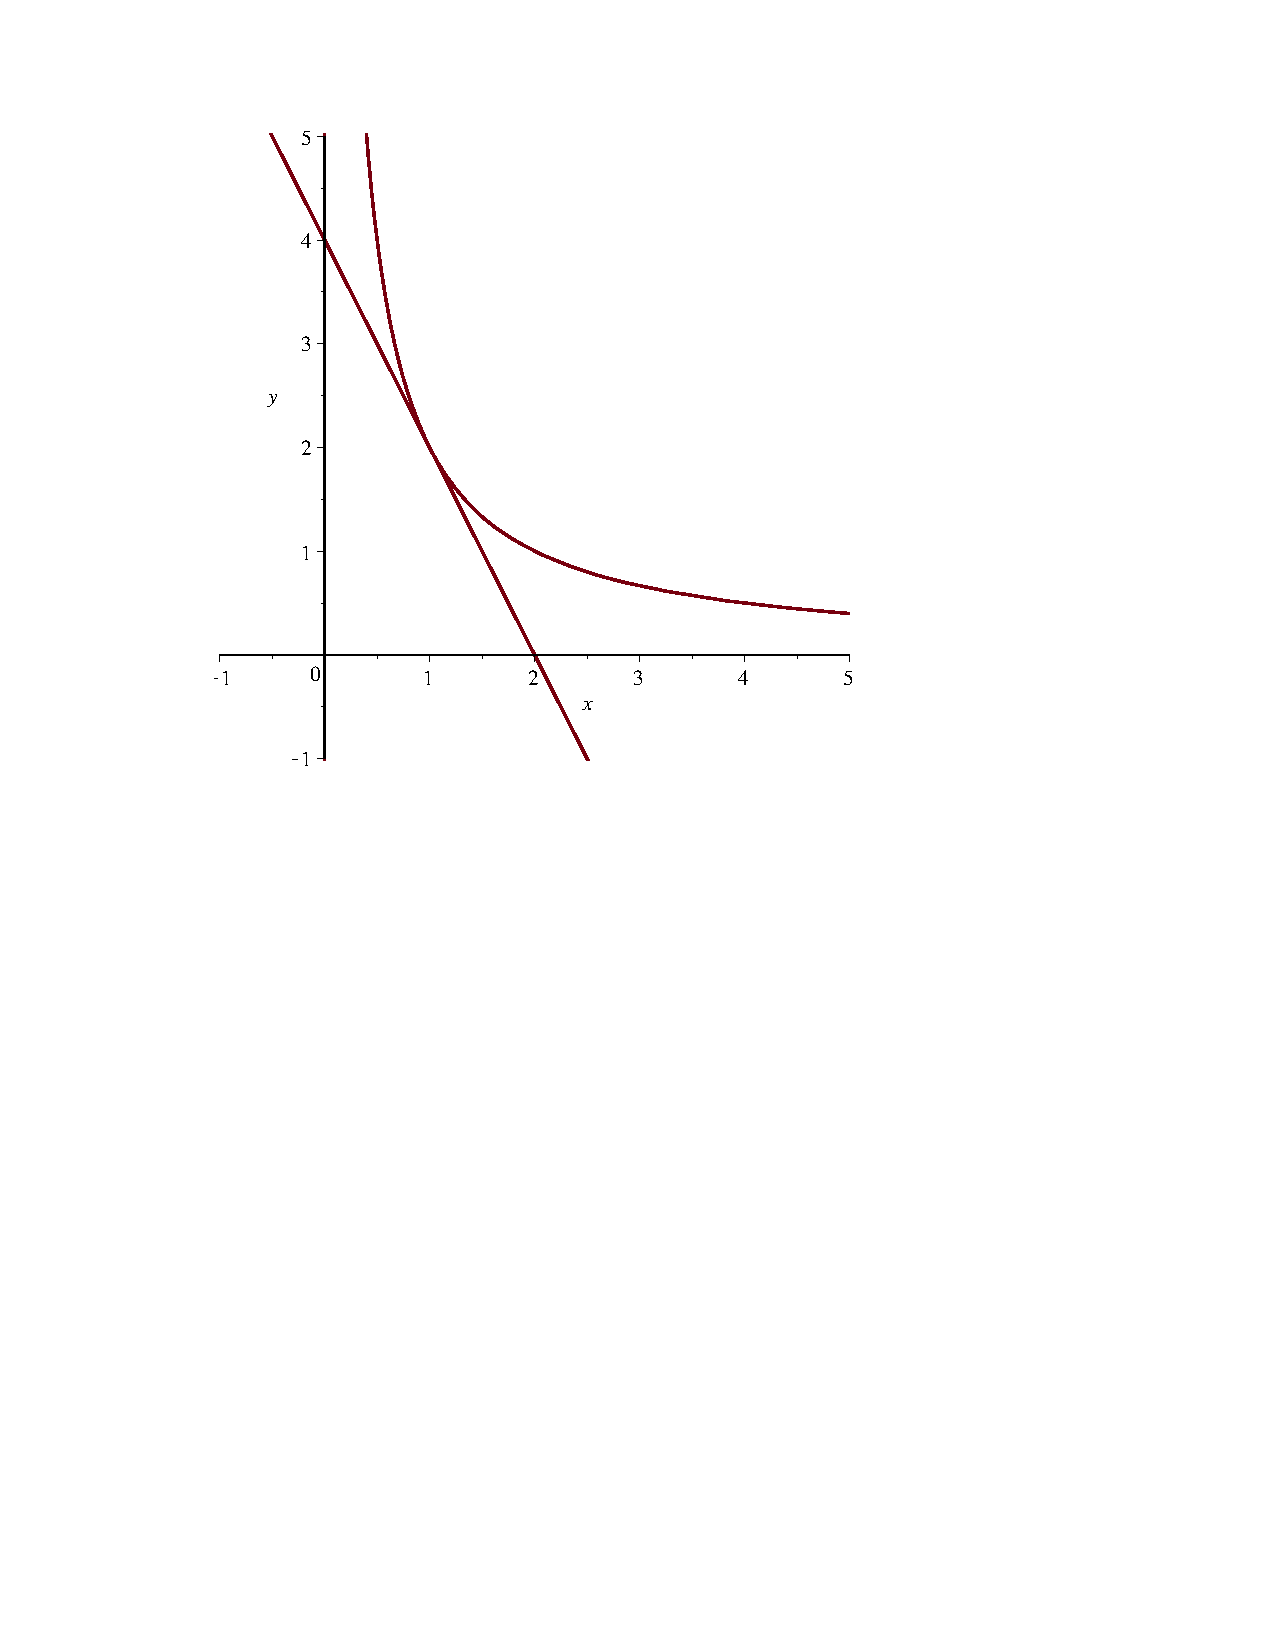
\includegraphics[scale=0.5]{graph.pdf}}} \fi

\item Show that the point of tangency bisects the segment of the tangent line (sketched in part b). i.e., show that the point of tangency is the midpoint of the segment of the tangent line which was sketched in part b.

\ifans{\fbox{\parbox{1\linewidth}{Note the x-intercept of the tangent line is $(2,0)$ and the $y$-intercept of the tangent line is $(0,4)$.\\

OPTION 1:\\
We can find the distance between the $x$-intercept and the point of tangency as well as the $y$-intercept and the point of tangency.  Specifically, the distance between the $x$-intercept of $(2,0)$ and the point of tangency of $(1,2)$ is $d=\sqrt{(x_2-x_1)^2+(y_2-y_1)^2}=\sqrt{(2-1)^2+(0-2)^2}=\sqrt{5}$.  Similarly, the distance between the $y$-intercept and the point of tangency can be shown to be $\sqrt{5}$.  So, the point of tangency is the midpoint of the two intercepts.\\

OPTION 2:\\
We can use the midpoint formula to find the midpoint of the line segment. $(x,y)=\left(\frac{x_1+x_2}{2},\frac{y_1+y_2}{2}\right)=\left(\frac{0+2}{2},\frac{4+0}{2}\right)=(1,2)$, which is the point of tangency.}}} \fi

\end{enumerate}

\item Show that the area of the triangle formed by any tangent line to the graph of $\displaystyle y=\frac{k}{x}$ and the coordinate axes is $2k$, for a fixed positive constant $k$.

\ifans{\fbox{\parbox{1\linewidth}{It can be shown that the equation of the tangent line to $\displaystyle f(x)=\frac{k}{x}$ at the point $x_0$ is $\displaystyle y-\frac{k}{x_0}=-\frac{k}{x_0^2}(x-x_0)$.  The $x$-intercept of this line is $\displaystyle \left(2x_0,0 \right)$ and the $y$-intercept of the tangent line is $\displaystyle \left(0,\frac{2k}{x_0}\right)$.  Thus, the base of the triangle has a length of $2x_0$ and the height of the triangle has a length of $\displaystyle \frac{2k}{x_0}$.  So, the area of the triangle is $\displaystyle A=\frac{1}{2}bh=\left(\frac{1}{2}\right) \left(2x_0\right) \left(\frac{2k}{x_0}\right)=2k$}}} \fi

\end{enumerate}

\end{document}